%! Licence = CC BY-NC-SA 4.0

%! Author = gianfluetsch
%! Date = 30. Dez 2021
%! Project = cydef_summary

\section{SPF/ KDIM/ DMARC \& RDP NLA}

\subsection{Overview}
\begin{center}
    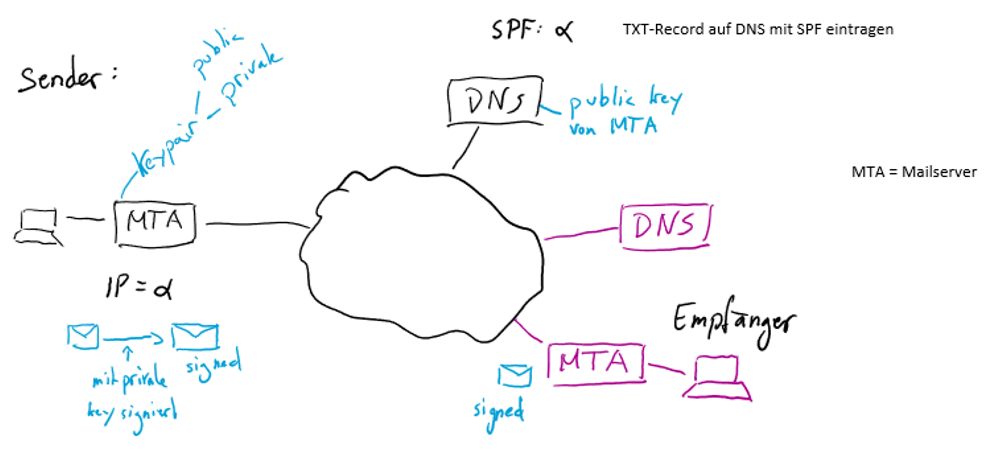
\includegraphics[width=1.0\linewidth]{spf_overview}
\end{center}

\textbf{SPF - Sender Policy Framework}\\
Auf dem \textbf{DNS} (schwarz) kann eingegrenzt werden, wer (welche IP) alles ein Mail verschicken darf.\\
\begin{itemize}
    \item \textcolor{OSTPink}{\textbf{MTA}} (violett) macht \textbf{DNS-Lookup} (schwarz) und fragt diesen an, welche IPs berechtig sind Mails zu versenden.\\
\end{itemize}
\begin{enumerate}
    \item IP-$\alpha$ (TCP) $\rightarrow$ DNS-Lookup $\rightarrow$ SPF@ost.ch
    \begin{enumerate}
        \item Falls $\alpha$ darin enthalten $\rightarrow$ ok\\
    \end{enumerate}
\end{enumerate}

Wenn Empfänger SPF-Policy nicht enforced, ist egal was der Sender konfiguriert hat. Empfänger-MTA interessiert das nicht.\\

\textcolor{cyan}{\textbf{DKIM - DomainKeys Identified Mail}}\\
\textit{DKIM} stellt einen Encryption Key und eine digitale Signatur bereit, die nachweisen, dass eine E-Mail-Nachricht nicht gefälscht oder verändert wurde.\\
\begin{itemize}
    \item Mailserver signiert mail mit private Key
    \item Mail kommt beim violetten MTA an und dieser prüft ob Mail signiert ist
    \begin{itemize}
        \item Wenn Signatur vorhanden $\rightarrow$ DNS-lookup (DNS schwarz) für public key $\rightarrow$ prüft Signatur von Mail mit dem public key des DNS Servers (schwarz)\\
    \end{itemize}
\end{itemize}

\textbf{DMARC - Domain-based Message Authentication, Reporting and Cornformance}\\
\textit{DMARC} vereinheitlicht die \textit{SPF}- und \textit{DKIM}-Authentifizierungsmechanismen in einem gemeinsamen Rahmen und ermöglicht es den Inhabern von Domänen, zu erklären, wie sie möchten, dass E-Mails von dieser Domäne behandelt werden, wenn sie einen Autorisierungstest nicht besteht.

\newpage

\subsection{Opportunistic TLS Encryption}
By checking the pcap files, one can see the \textit{STARTTLS} messages which will let us know tls encryption has been used.

\begin{center}
    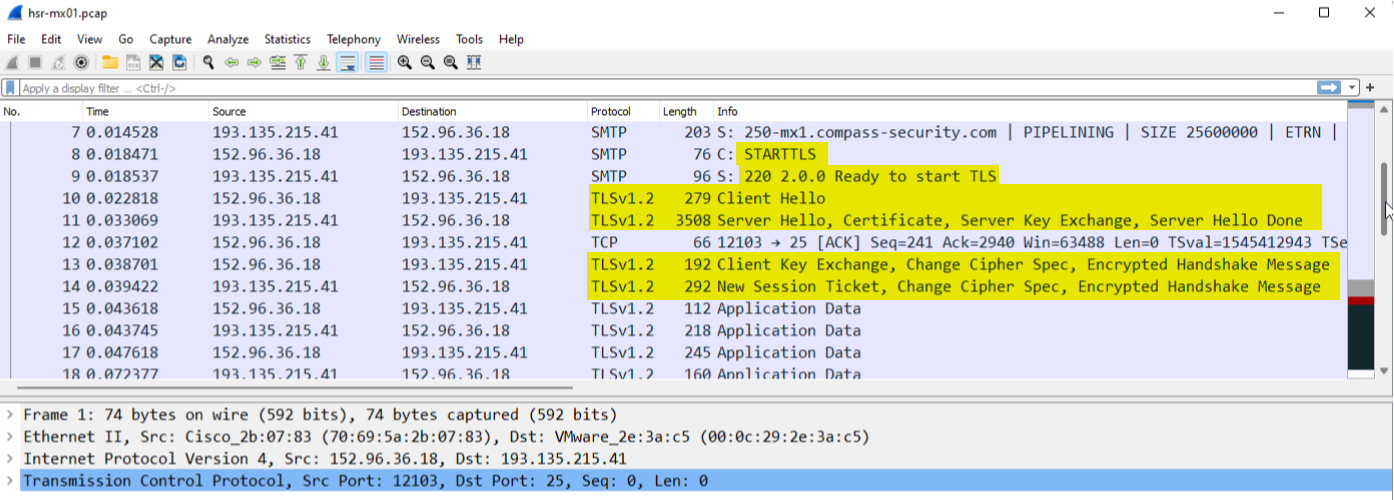
\includegraphics[width=1.0\linewidth]{tls_encryption}
\end{center}

\subsection{SPF}
Wenn \textit{SPF} (Sender Policy Framework) verwendet wird, sollte dies im Header/ Log ersichtlich sein!
\begin{center}
    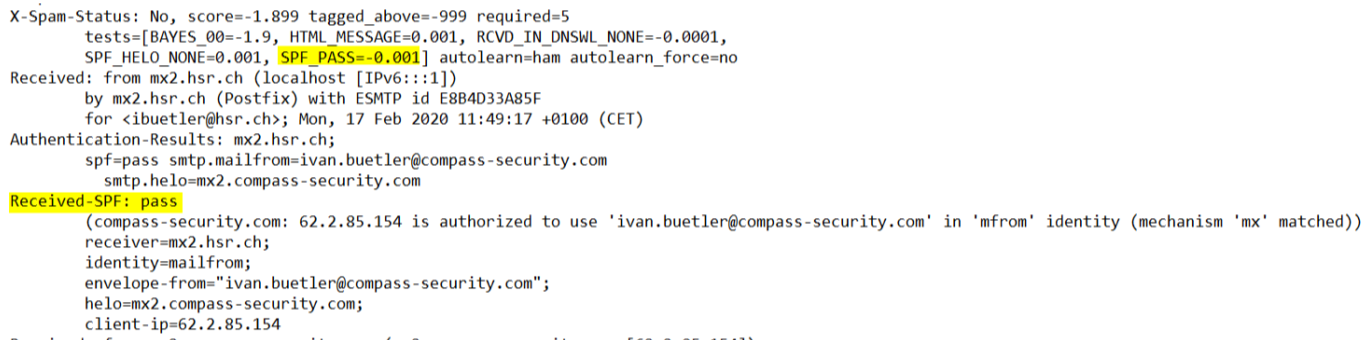
\includegraphics[width=1.0\linewidth]{spf}
\end{center}
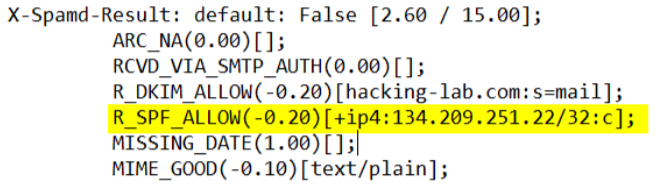
\includegraphics[width=0.3\linewidth]{spf2}
\begin{center}
    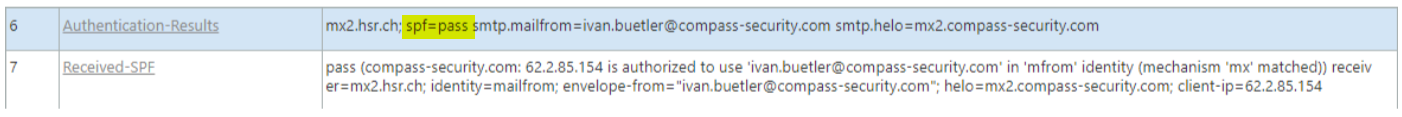
\includegraphics[width=1.0\linewidth]{spf3}
\end{center}

\newpage

\subsection{DKIM}
Wenn \textit{DKIM} (DomainKeys Identified Mail) verwendet wird, sollte dies im Header/ Log ersichtlich sein!

\begin{center}
    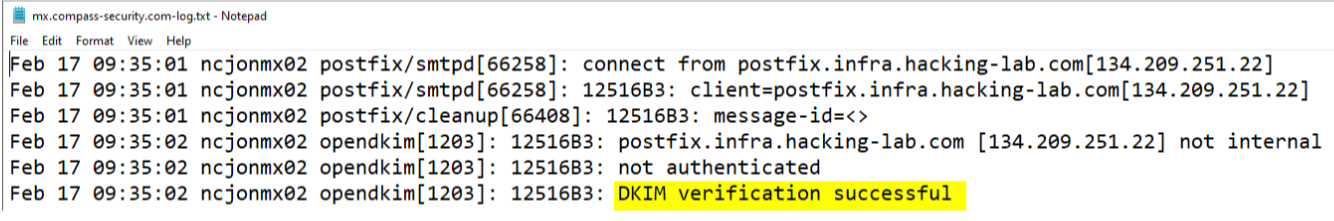
\includegraphics[width=1.0\linewidth]{dkim}
\end{center}

Due to the MX of Compass, the \textit{DKIM} service is initialized. But the headers from the OWA doe not have DKIM headers applied. Thus, DKIM isn't used!

\begin{center}
    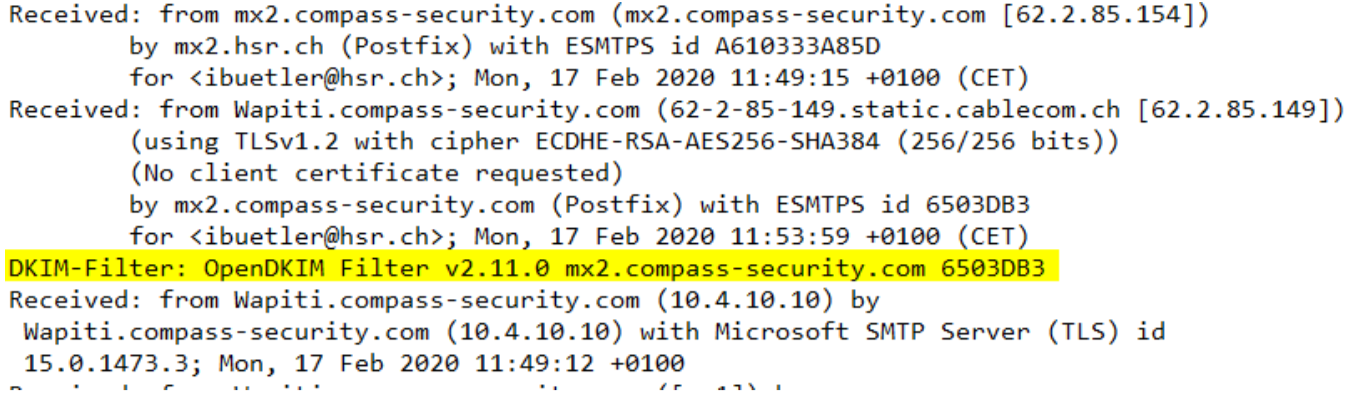
\includegraphics[width=0.8\linewidth]{dkim2}
\end{center}

\subsection{DMARC}
\textit{DMARC} (Domain-based Message Authentication) is available!

\begin{center}
    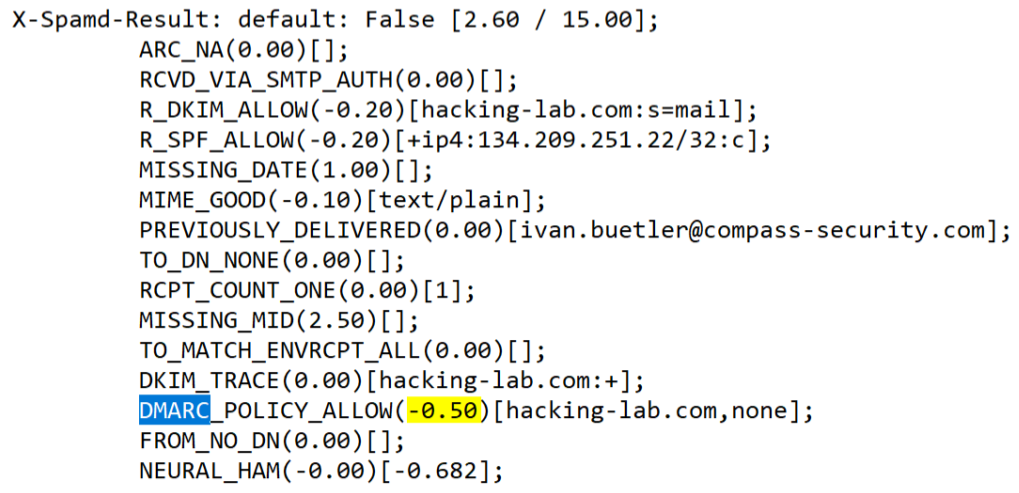
\includegraphics[width=0.6\linewidth]{dmarc}
\end{center}

DMARC not available (NA)!
\begin{center}
    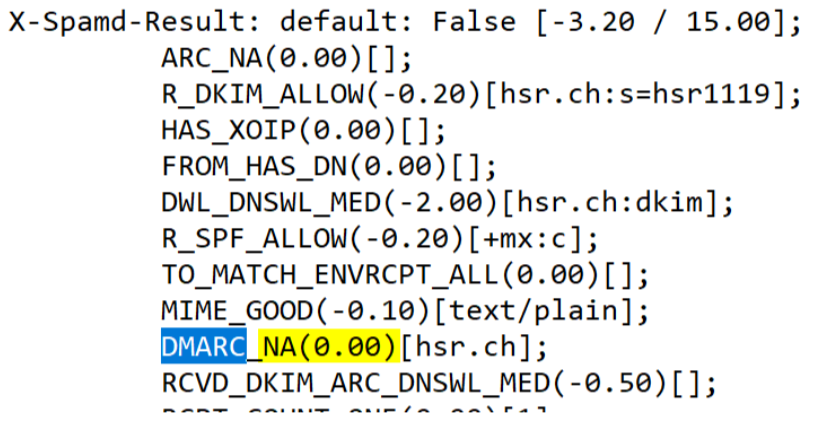
\includegraphics[width=0.4\linewidth]{dmarc2}
\end{center}

\newpage

\subsection{RDP NLA}

\subsubsection{Explain NLA}
\textit{NLA} (Network Level Authentication) is an authentication tool used in Remote Desktop Services or Remote Desktop Connection.
\textit{NLA} moves the authentication aspect of a remote session from the RDP layer to the network layer. The use of \textit{NLA} is recommended to reduce the attack surface of systems exposed to the RDP protocol.

\textit{NLA} only works with \textbf{challenge-response-authentication protocols}.

\subsubsection{Explain CredSSP}
Credential Security Support Provider (\textit{CredSSP}) allows credentials to be forwarded to a remote host, where they are then used for authentication. Well-known applications that use this method are the RDP client or PowerShell. For the latter, \textit{CredSSP} can solve the second-hop problem when connecting to another remote host from a remote session.

\subsubsection{RDP MitM}
\begin{center}
    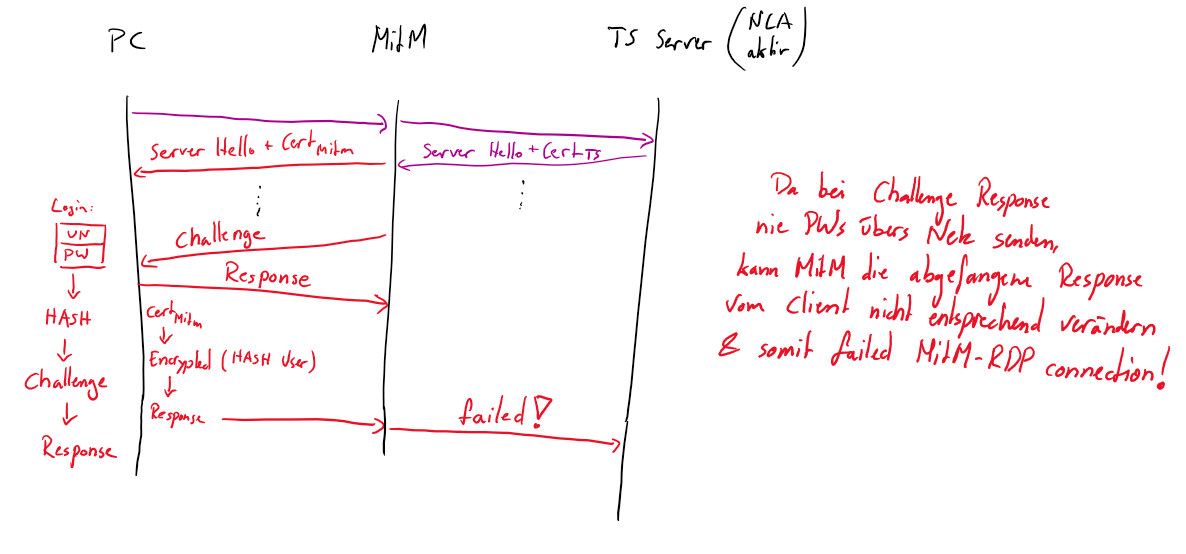
\includegraphics[width=1.0\linewidth]{rdp_mitm}
\end{center}

\textbf{Dies geht aber nur bei \textit{Challenge-Response} Verfahren!!}\\
$\rightarrow$ sobald Passwort übers Netz übermittelt wird, würde MitM wieder funktionieren

\subsubsection{Explain why NLA should protect against MitM}
If a client wants to establish an RDP connection to a terminal server (TS), a MitM could hang itself between this connection.
The MitM forwards the client's request to the server. The server responds with a \textit{Server Hello + the Cert of the TS}. This response is now forwarded to the client with the \textit{Cert of the MitM} instead of the \textit{Cert of the TS}. The client now responds with a \textit{Client Hello}, etc.

Finally the TS sends a challenge to the client (via the MitM). The client now encrypts the hash of the user (\textit{Hash via username + password}) together with the received \textit{cert of the MitM}. The client now sends this response to the MitM. The MitM would have to modify this response so that the encryption is done with the \textit{TS-Cert} and no longer with the \textit{MitM-Cert}. Since passwords are never sent over the network in the challenge response, the MitM can't modify this response as necessary.
Thus the RDP connection between the MitM and the server cannot be established.

\newpage

\subsubsection{Would 2FA fix the problem of this kind of MitM attack?}
\textit{2FA} brings no advantage with \textit{MitM}, because if the 2nd factor is confirmed (which the MitM does not intercept), the connection is ultimately established via the MitM anyway.
Since MitM attacks are no longer possible with NLA, 2FA is not necessary to minimize this attack.

\textit{2FA} will not fix the fundamental problem of \textit{MitM}, but the attacker can only hijack the victim if the victim is logging into the target server via \textit{MitM}. Mutual Auth would really solve the issue!

\subsubsection{Mutual Authentication (Challenge-Response)}
\textcolor{red}{\textbf{Passwort geht nie übers Netz (nur der Hash des Passwortes)}}\\

\begin{minipage}{0.45\linewidth}
    \begin{enumerate}
        \item Client $\rightarrow$ Server: \textit{Anfrage}
        \item Server $\rightarrow$ Client: \textit{generiert Challenge}
        \item Client $\rightarrow$ Server: \textit{generiert Response auf Challenge (mit dem Hash seines Passwortes)}
        \item Server $\rightarrow$ Client: \textit{Server prüft Response auf eigene Antwort auf Challenge anhand selber generierter Response mit gespeichertem Hash des PWs}
    \end{enumerate}
\end{minipage}
\begin{minipage}{0.5\linewidth}
    \begin{center}
        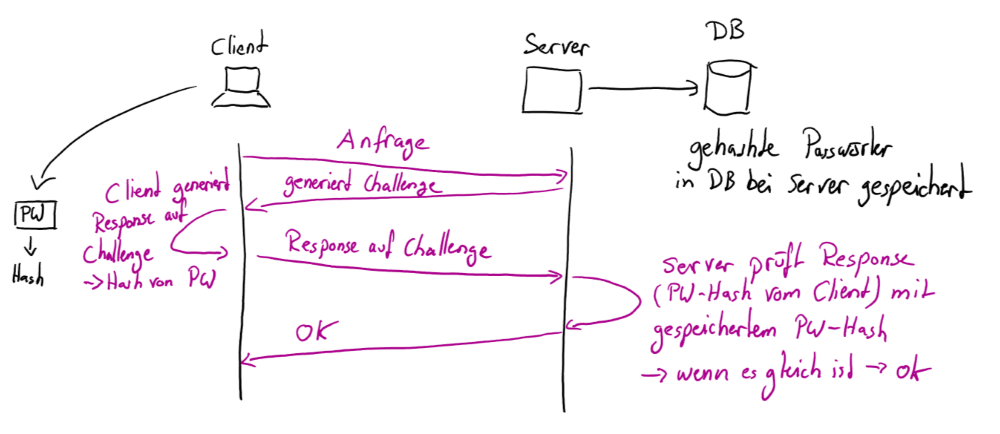
\includegraphics[width=1.0\linewidth]{challenge_response}
        \vspace{-8pt}
    \end{center}
\end{minipage}

\subsubsection{What is the difference between the two nmap outputs in the steps above (enabled/disabled NLA)?}
As you can see below with \textbf{enabled NLA} the nmap output shows \textit{no SSL} (but RDSTLS), in contrast to \textbf{disabled NLA} where SSL is displayed as enabled (in addition to \textit{RDSTLS}).

\begin{lstlisting}[language=bash]
    # disabled NLA
    nmap -P0 -p 3389 --script rdp-enum-encryption 192.168.6.128
    Host discovery disabled (-Pn). All addresses will be marked 'up' and scan times will be slower.
    Starting Nmap 7.91 ( https://nmap.org ) at 2021-11-10 15:37 CET
    Nmap scan report for 192.168.6.128
    Host is up (0.00052s latency).
    
    PORT     STATE SERVICE
    3389/tcp open  ms-wbt-server
    | rdp-enum-encryption:
    |   Security layer
    |     CredSSP (NLA): SUCCESS
    |     CredSSP with Early User Auth: SUCCESS
    |     RDSTLS: SUCCESS
    |     SSL: SUCCESS
    |_  RDP Protocol Version: Unknown
    MAC Address: 00:0C:29:50:EB:DA (VMware)
    
    Nmap done: 1 IP address (1 host up) scanned in 1.75 seconds
\end{lstlisting}

\begin{lstlisting}[language=bash]
    # enabled NLA
    nmap -P0 -p 3389 --script rdp-enum-encryption 192.168.6.128
    Host discovery disabled (-Pn). All addresses will be marked 'up' and scan times will be slower.
    Starting Nmap 7.91 ( https://nmap.org ) at 2021-11-10 15:36 CET
    Nmap scan report for 192.168.6.128
    Host is up (0.00036s latency).
    
    PORT     STATE SERVICE
    3389/tcp open  ms-wbt-server
    | rdp-enum-encryption:
    |   Security layer
    |     CredSSP (NLA): SUCCESS
    |     CredSSP with Early User Auth: SUCCESS
    |_    RDSTLS: SUCCESS
    MAC Address: 00:0C:29:50:EB:DA (VMware)
    
    Nmap done: 1 IP address (1 host up) scanned in 1.75 seconds
\end{lstlisting}

\subsubsection{SSL Success (deaktiviertes NLA) - RSTLS (aktiviertes NLA)}

Richtig zur Sache geht es, wenn man die erlaubten Security- und Verschlüsselungsmodi abfragt. Das sieht dann im Idealfall eines fest auf NLA eingestellten RDP-Systems so aus:

\begin{lstlisting}[language=bash]
    nmap -P0 -p 3389 --script rdp-enum-encryption 192.168.6.16
    ...
    | rdp-enum-encryption:
    |   Security layer
    |     CredSSP (NLA): SUCCESS
    |     CredSSP with Early User Auth: SUCCESS
    |_   RDSTLS: SUCCESS
\end{lstlisting}

Erlaubt ist nur \textit{Enhanced RDP Security mit CredSSP} und ein spezieller Modus namens \textit{RDSTLS}, der für zwischen geschaltete RDP-Gateways zum Einsatz kommt. Doch auf vielen Systemen sieht das Ergebnis eher so aus:

\begin{lstlisting}[language=bash]
    |   Security layer
    |     CredSSP (NLA): SUCCESS
    |     CredSSP with Early User Auth: SUCCESS
    |     Native RDP: SUCCESS
    |     RDSTLS: SUCCESS
    |     SSL: SUCCESS
    |   RDP Encryption level: High
    |     40-bit RC4: SUCCESS
    |     56-bit RC4: SUCCESS
    |     128-bit RC4: SUCCESS
    |     FIPS 140-1: SUCCESS
    |_  RDP Protocol Version:  RDP 5.x, 6.x, 7.x, or 8.x server
\end{lstlisting}

Also in anderen Worten: \glqq anything goes\grqq. Dieser Server bietet nicht nur Enhanced Security mit NLA, die zwar bevorzugt wird, sondern auch die kaputte Standard RDP Security mit ihren nutzlosen Krypto-Verfahren, die dann zum Einsatz kommt, wenn der Client sie explizit anfordert. Was ein Angreifer natürlich genau so tun würde.

Problematisch ist übrigens auch die Zeile \lstinline|SSL: SUCCESS|. RDPs Enhanced Security gestattet es nämlich nach wie vor, auf die vorgeschaltetete Network Level Authentication (NLA) zu verzichten und die klassische Anmeldung via Windows-Login lediglich mit einem TLS-Tunnel zu versehen (der dann die selber gebastelte RDP-Encryption von Microsoft ersetzt).

